% inkscape image.pdf --export-type=png --export-filename=image.png --export-width=1024 --export-background-opacity=0
% \documentclass[a3paper]{article}
% \usepackage[left=0mm,top=1cm,right=0mm,bottom=0mm]{geometry}
\documentclass[border=0]{standalone}
% \documentclass[dvisvgm]{minimal}
\usepackage{tikz}
\usetikzlibrary{calc,lindenmayersystems}
\usepackage{xcolor}
\definecolor{pGreen}{HTML}{663366}
\begin{document}
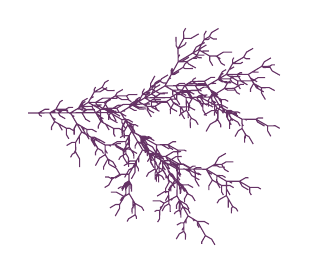
\begin{tikzpicture}
\draw[pGreen, rotate=0]
[l-system={rule set={F -> FF-[-F+F]+[+F-F]}, axiom=F, order=4, step=2pt,
randomize step percent=25, angle=30, randomize angle percent=5}]
lindenmayer system;
\end{tikzpicture}
\end{document}